\section{校正理論}
作用力測定装置から得た抗力方向および揚力方向における出力電圧$V_D$,$V_L$を
正規座標系の$x$軸方向および$y$軸方向の荷重$v_x$,$v_y$に換算する際に,
出力電圧$V_D$,$V_L$と$v_x$,$v_y$の関係性を明らかにするための校正実験を
行う必要がある.
校正実験によって得られた結果を用いて関係性を明らかにするための校正理論について述べる.

\subsection{作用力測定装置と校正実験装置の関係}
はじめに,作用力測定装置と校正実験装置の関係について説明する.

作用力測定装置と校正実験装置の設置位置によって校正実験結果は大きく変動するため,
その影響を考慮し,補正処理を行う必要がある.
このとき以下のような要因が,校正実験結果への影響を与えていると考えられる.

\begin{enumerate}[(1)]
    \item 作用力測定装置にひずみセンサが正確に取り付けることが難しい
    \item 作用力測定装置が回流水槽に正確に設置することが難しい
    \item 作用力測定装置と校正装置の回転軸を一致させることが難しい
\end{enumerate}

ここで,水流に対する座標系を正規座標系 $(x,y)$,
作用力測定装置の座標系を座標系(1) $(x',y')$,
校正装置の座標系を座標系(2) $(x,'' y'')$とする.

このとき,(1) 作用力測定装置にひずみセンサを正確に取り付けることが難しいこと,
(2) 作用力測定装置が回流水槽に正確に設置することが難しいことから,
座標系[1]は正規座標系に対して
$x'$軸は$x$軸から$\theta_x1$,$y'$軸は$y$軸から$\theta_y1$だけ回転している.
また,座標系[2]は正規座標系に対して
$x''$軸は$x$軸から$y$方向に$\Delta x$,
$y''$軸は$y$軸から$x$方向に$\Delta y$だけオフセットを持つ状態となる.

\newpage

\subsection{出力電圧勾配}

作用力測定装置を評価にあたり,作用力測定装置に取り付けられた2組のひずみセンサ
および校正実験の際に作用力を与えるロードセルの出力電圧の対応関係を調べることで評価を行う.
ここで,作用力測定装置において抗力方向のひずみセンサの出力電圧を$V_d$,揚力方向を$V_l$,
ロードセルの出力電圧を$V$とするとき,抗力方向の出力電圧勾配を$v_d$,
揚力方向の出力電圧勾配を$v_l$とすると以下のように表すことができる.

\begin{align}
    v_d = V_d / V\\
    v_l = V_l / V
\end{align}

\subsection{座標系の回転における補正理論}

正規座標系と座標系[1]の回転における補正理論を説明する.
ここでは,座標系のオフセットはない($\Delta x = 0$,$\Delta y = 0$)として考える.
上述の通り正規座標系と座標系[1]について,以下のFig.のように回転角$\theta_{x1}$,$\theta_{y1}$を持つ.
ここで,作用力$F_1$を与えるとそれぞれの方向に作用力$F_{x1}$,$F_{y1}$,$F_{x'1}$,$F_{y'1}$が加わる.
このとき,作用力測定装置から得られる電圧$V_{d1}$,$V_{l1}$は作用力$F_{x'1}$,$F_{y'1}$に起因するものである.
また,得られた出力電圧$V_{d1}$,$V_{l1}$および$V_{x'1}$,$V_{y'1}$から,ロードセルの出力電圧$V_1$を用いて
出力電圧勾配$v_{d1}$,$v_{l1}$および$v_{x'1}$,$v_{y'1}$をm止めることができる.
したがって,正規座標系と座標系[1]の関係について,
$v_{x1}$と$v_{x'1}$および$v_{y1}$と$v_{y'1}$の関係を明らかにすれば良い,

\subsection{回転角$\theta_{x1}$,$\theta_{y1}$の算出}
はじめに,回転角$\theta_{x1}$,$\theta_{y1}$を算出する.
理論式における$v_{x\;Theory}$及び$v_{y\;Theory}$は正弦波とその位相差で表すことができる.
したがって,校正実験結果の各角度の出力電圧勾配においても同様の正弦波と
その位相差で表すことが可能であると予想することができる.
このとき,離散フーリエ変換を適用し,
波数1の成分について,実部を$Re$,虚部を$Im$として
位相角$\phi$を求めることができる.

\begin{align}
    \phi = \arctan \left(\frac{Im}{Re}\right) \cdot \frac{180}{\pi}
\end{align}
\vskip \baselineskip

抗力方向の結果から得られた位相角を$\phi_1$,揚力方向から得られた位相角を$\phi_2$と
するとき,抗力方向の出力電圧勾配$v_d$と
正規座標系における$x$軸方向の出力電圧勾配の理論値$v_{x\; Theory}$との位相差
$\theta_1$,
揚力方向の出力電圧勾配$v_l$と
正規座標系における$y$軸方向の出力電圧勾配の理論値$v_{y\; Theory}$との位相差
$\theta_2$は以下のように表される.

\begin{align}
    \theta_1 = \pi - \phi_1\\
    \theta_2 = \frac{\pi}{2} - \phi_2
\end{align}
\vskip \baselineskip

したがって,$x'$軸,$y'$軸は左回りを正方向として,それぞれ$\theta_1$,$\theta_2$だけ
回転していることとなる.
また,作用力測定装置に取り付けられた抗力・揚力方向のひずみセンサの取付角$\phi_s$は
位相角$\phi_1$,$\phi_2$より求めることができる.

\begin{align}
    \phi_s = \left| \phi_1 - \phi_2 \right|
\end{align}

\subsection{出力電圧勾配の座標変換}
位相角$\theta_1$,$\theta_2$が求められたことから,
それらを用いて出力電圧勾配の座標変換を行う.
ここで,座標系[1]の$x'$軸,$y'$軸を
それぞれ$f_{x1}\left(x\right)$,$f_{y1}\left(x\right)$として,
正規座標軸の$x$を用いた式で表す.

算出した位相角$\theta_1$,$\theta_2$より,$f_{x1}\left(x\right)$,$f_{y1}\left(x\right)$は
以下のように表される.

\begin{align}
    f_{x1}\left(x\right) &= \tan \theta_1 \; x\\
    f_{y1}\left(x\right) &= - \frac{1}{\tan \theta_2}\; x
\end{align}
\vskip \baselineskip

このとき,作用力$F_1$は,Fig.に示す点$F_1$の座標を表すベクトルと考えることができる.
また,その座標はFig.より,$f_{x1}\left(x\right)$,$f_{y1}\left(x\right)$の法線で,
点$v_{x'1}$,$v_{y'1}$を通る直線,
$f_{x2}\left(x\right)$,$f_{y2}\left(x\right)$の交点であることがわかる.\par
ここで,ひずみゲージから得ることのできる出力電圧の傾きから,
$v_{x'1}$,$v_{y'1}$のベクトルの大きさ$|\boldsymbol{v_{x'1}}|$,$|\boldsymbol{v_{y'1}}|$を
得ることができる.
角度$\theta_1$,$\theta_2$が求められていることから,
点$v_{x'1}$,$v_{y'1}$の座標は以下のように求めることができる.

\begin{align}
    v_{x'1} \left(x ,y\right) &= \left(|\boldsymbol{v_{x'1}}| \cos \theta_1,\; |\boldsymbol{v_{x'1}}| \sin \theta_2\right)\\
    v_{y'1} \left(x ,y\right) &= \left( - |\boldsymbol{v_{y'1}}| \sin \theta_1,\; |\boldsymbol{v_{y'1}}| \cos \theta_2\right)
\end{align}
\vskip \baselineskip

次に,直線$f_{x2}\left(x\right)$,$f_{y2}\left(x\right)$を求める.
$f_{x1}\left(x\right)$,$f_{y1}\left(x\right)$,点$v_{x'1}$,$v_{y'1}$の座標から
それぞれ以下のように算出される.

\begin{align}
    f_{x2}\left(x\right) &= - \frac{1}{\tan \theta_1} \; x + \frac{|v_{x'}|}{\sin \theta_1}\\
    f_{y2}\left(x\right) &= \tan \theta_2\; x + \frac{|v_{y'}|}{\cos \theta_2}
\end{align}
\vskip \baselineskip

以上の$f_{x2}\left(x\right)$,$f_{y2}\left(x\right)$から,
交点の座標$F_1\left(x,y\right)$を求めると以下のようになる.

\begin{align}
    x &= \frac{v_{x'1} \cos \theta_2 - v_{y'1} \sin \theta_1}{\sin \theta_1 \sin \theta_2 + \cos \theta_1 \cos \theta_2}\\          
    y &= - \frac{1}{\tan \theta_1} \; \left(\frac{v_{x'1} \cos \theta_2 - v_{y'1} \sin \theta_1}{\sin \theta_1 \sin \theta_2 + \cos \theta_1 \cos \theta_2}\right) + \frac{|v_{x'1}|}{\sin \theta_1}\\
    &= \tan \theta_2\; \left(\frac{v_{x'1} \cos \theta_2 - v_{y'1} \sin \theta_1}{\sin \theta_1 \sin \theta_2 + \cos \theta_1 \cos \theta_2}\right) + \frac{|v_{y'}|}{\cos \theta_2}
\end{align}  
\vskip \baselineskip

したがって,正規座標系における$x$軸方向の出力電圧勾配$v_x$および揚力方向の$v_y$は,以下のように表される.

\begin{align}
    v_x &= \frac{v_{x'} \cos \theta_2 - v_{y'} \sin \theta_1}{\sin \theta_1 \sin \theta_2 + \cos \theta_1 \cos \theta_2}\\          
    v_y &= - \frac{1}{\tan \theta_1} \; \left(\frac{v_{x'} \cos \theta_2 - v_{y'} \sin \theta_1}{\sin \theta_1 \sin \theta_2 + \cos \theta_1 \cos \theta_2}\right) + \frac{|v_{x'}|}{\sin \theta_1}\\
    &= \tan \theta_2\; \left(\frac{v_{x'} \cos \theta_2 - v_{y'} \sin \theta_1}{\sin \theta_1 \sin \theta_2 + \cos \theta_1 \cos \theta_2}\right) + \frac{|v_{y'}|}{\cos \theta_2}
\end{align}
\vskip \baselineskip

以上の過程より,座標系[1]から正規座標系への変換が可能である.

\newpage

\subsection{補正理論のテストデータへの適用 (1)}

上記の座標系の回転における補正理論の有用性を確かめるために,
以下の式から,任意の回転角$\theta_{1\;\mathrm{test}}$,$\theta_{2\; \mathrm{test}}$を与えて
出力電圧勾配について抗力方向を$v_{x\;\mathrm{test}}$,揚力方向を$v_{y\;\mathrm{test}}$
として,テストデータを作成した.

\begin{align}
    v_{x\;\mathrm{test}} \left(i\right) &= \cos \left( \frac{\pi}{24}\; i + \pi - \theta_{1\;\mathrm{test}} \right)\\
    v_{y\;\mathrm{test}} \left(i\right) &= \cos \left( \frac{\pi}{24}\; i + \frac{1}{2} \pi - \theta_{2\;\mathrm{test}} \right) \; \left(i = 1,2,3,\cdots\right)
\end{align}
\vskip \baselineskip

また,今回は以下のTable のようなパラメータを用いた.

\begin{table}[htbp]
    \begin{center}
        \caption{Test data conditions}
        \begin{tabular}{|p{30mm}|p{20mm}|p{30}|}
            \hline
            \multicolumn{1}{|c|}{} & \multicolumn{1}{|c|}{\textgt{$\theta_{1\mathrm{test}}$ [deg]}}   & \multicolumn{1}{|c|}{$\theta_{2\mathrm{test}}$ [deg]}                 \\ \hline
            \multicolumn{1}{|c|}{Case 1}      & \multicolumn{1}{|c|}{15}  & \multicolumn{1}{|c|}{20} \\ \hline
            \multicolumn{1}{|c|}{Case 2}      & \multicolumn{1}{|c|}{-15}  & \multicolumn{1}{|c|}{-20}       \\ \hline
            \multicolumn{1}{|c|}{Case 3}      & \multicolumn{1}{|c|}{15}  & \multicolumn{1}{|c|}{-20}       \\ \hline
            \multicolumn{1}{|c|}{Case 4}      & \multicolumn{1}{|c|}{90}  & \multicolumn{1}{|c|}{-90}       \\ \hline
        \end{tabular}
    \end{center}
\end{table}


このとき,作成されたテストデータの図および補正適用後の図は以下のFig.~Fig. のようになる.

\begin{multicols}{2}

    \begin{figure_here}
    \subsubsection{テストデータ : Case 1}
    \vskip \baselineskip
    $\theta_{1 \mathrm{test}} = 15 \; \mathrm{[deg]}$, $\theta_{2 \mathrm{test}} = 20 \; \mathrm{[deg]}$
        \footnotesize
        \begin{center}
            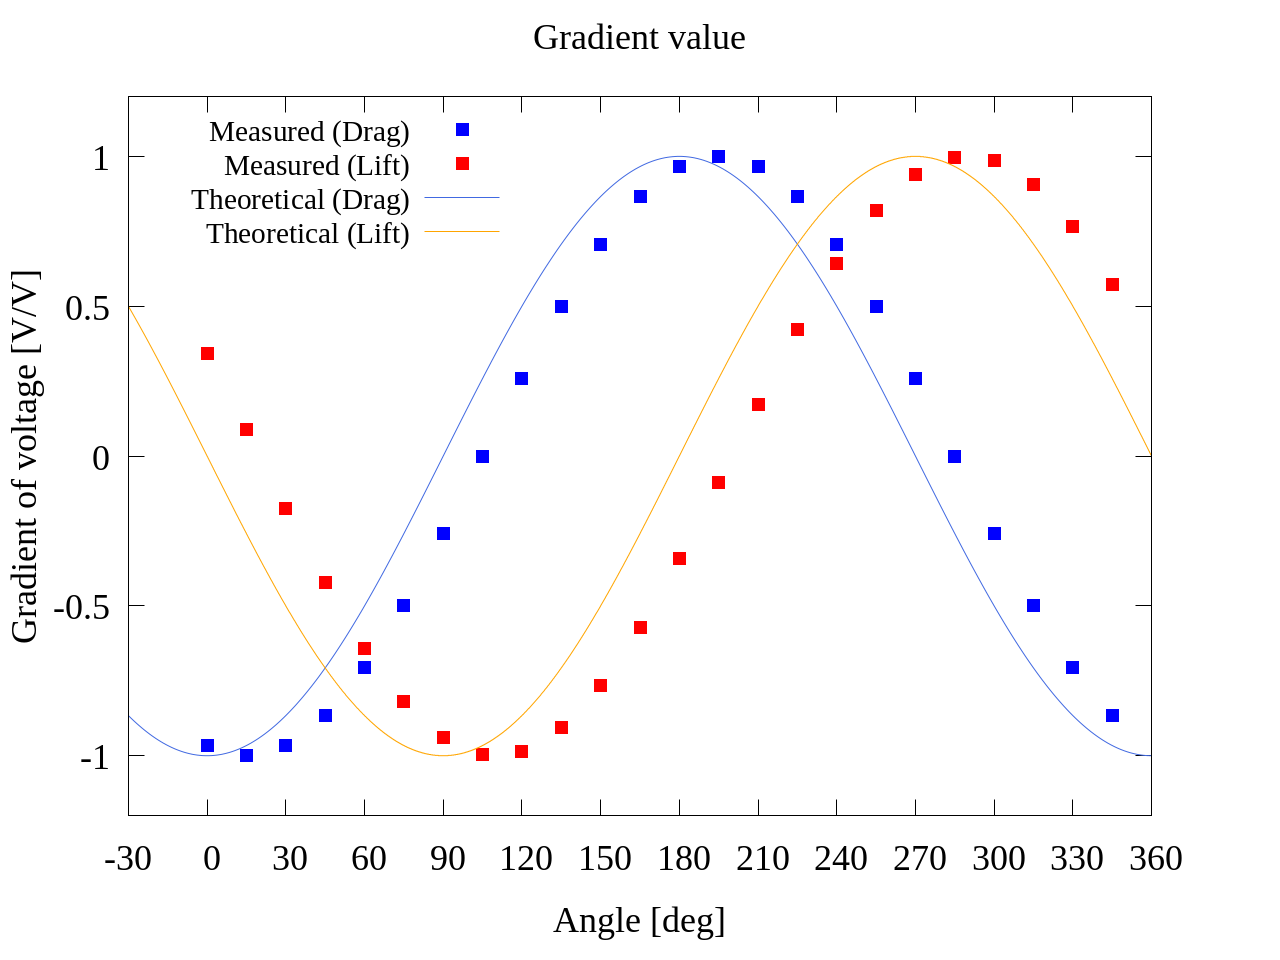
\includegraphics[width=65mm]{../../02_workspace/result/rotation_tx=15.0_tx=20.0/plot/20/20_adjust-value.png}
            \caption{Simulated data [Case 1]}
            \includegraphics[width=65mm]{../../02_workspace/result/rotation_tx=15.0_tx=20.0/plot/21/21-4_corrected_angle_drag.png}
            \caption{Corrected data (Drag) [Case 1]}
            \includegraphics[width=65mm]{../../02_workspace/result/rotation_tx=15.0_tx=20.0/plot/21/21-4_corrected_angle_lift.png}
            \caption{Corrected data (Lift) [Case 1]}
        \end{center}
    \end{figure_here}

    \begin{figure_here}
        \subsubsection{テストデータ : Case 2}
        \vskip \baselineskip
        $\theta_{1 \mathrm{test}} = -15 \; \mathrm{[deg]}$, $\theta_{2 \mathrm{test}} = -20 \; \mathrm{[deg]}$
        \footnotesize
        \begin{center}
            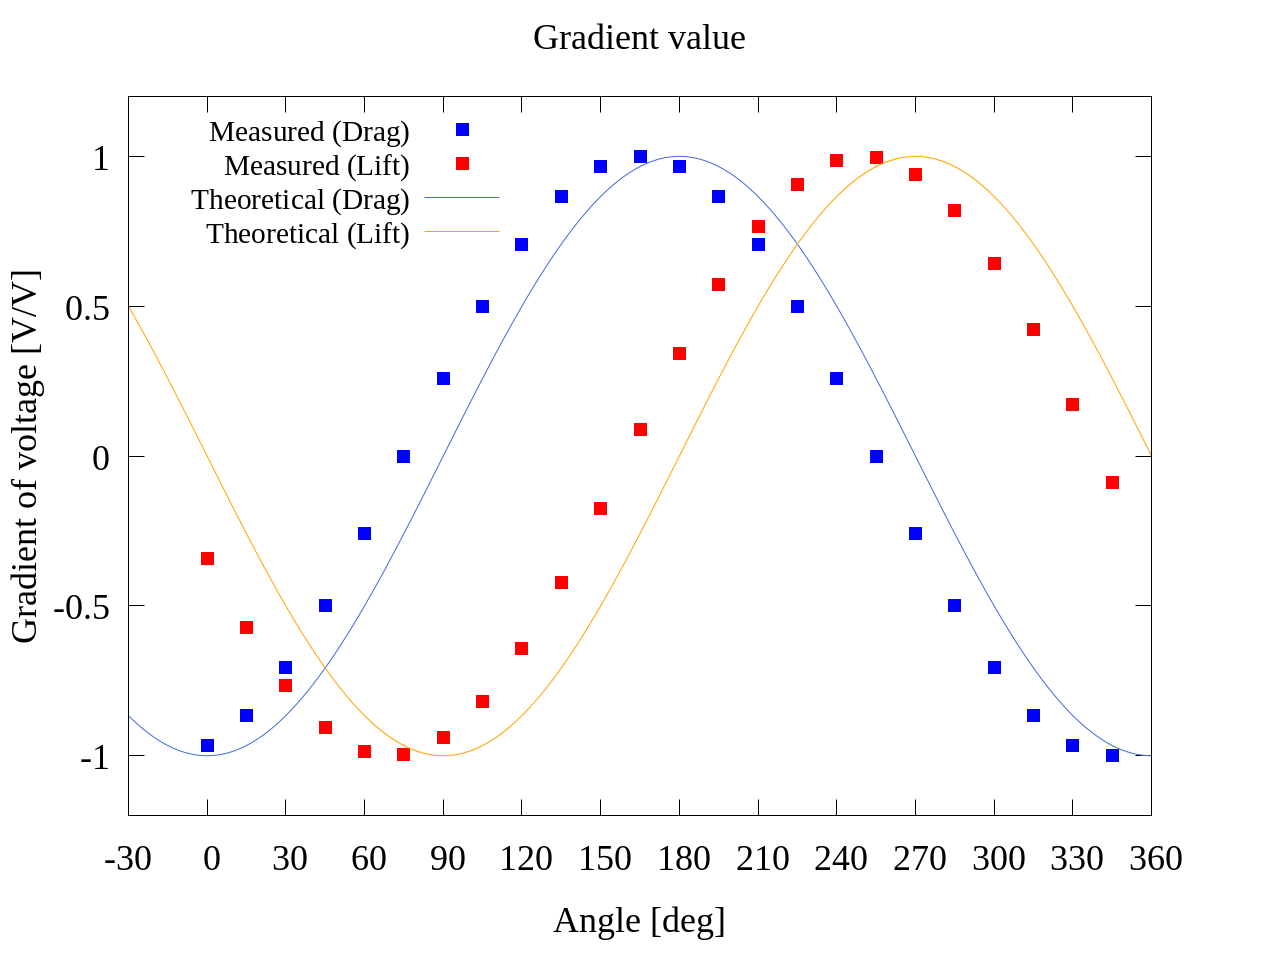
\includegraphics[width=65mm]{../../02_workspace/result/rotation_tx=-15.0_tx=-20.0/plot/20/20_adjust-value.png}
            \caption{Simulated data [Case 2]}
            \includegraphics[width=65mm]{../../02_workspace/result/rotation_tx=-15.0_tx=-20.0/plot/21/21-4_corrected_angle_drag.png}
            \caption{Corrected data (Drag) [Case 2]}
            \includegraphics[width=65mm]{../../02_workspace/result/rotation_tx=-15.0_tx=-20.0/plot/21/21-4_corrected_angle_lift.png}
            \caption{Corrected data (Lift) [Case 2]}
        \end{center}
    \end{figure_here}

\newpage

    \begin{figure_here}
        \subsubsection{テストデータ : Case 3}
        \vskip \baselineskip
        $\theta_{1 \mathrm{test}} = 15 \; \mathrm{[deg]}$, $\theta_{2 \mathrm{test}} = -20 \; \mathrm{[deg]}$
        \footnotesize
        \begin{center}
            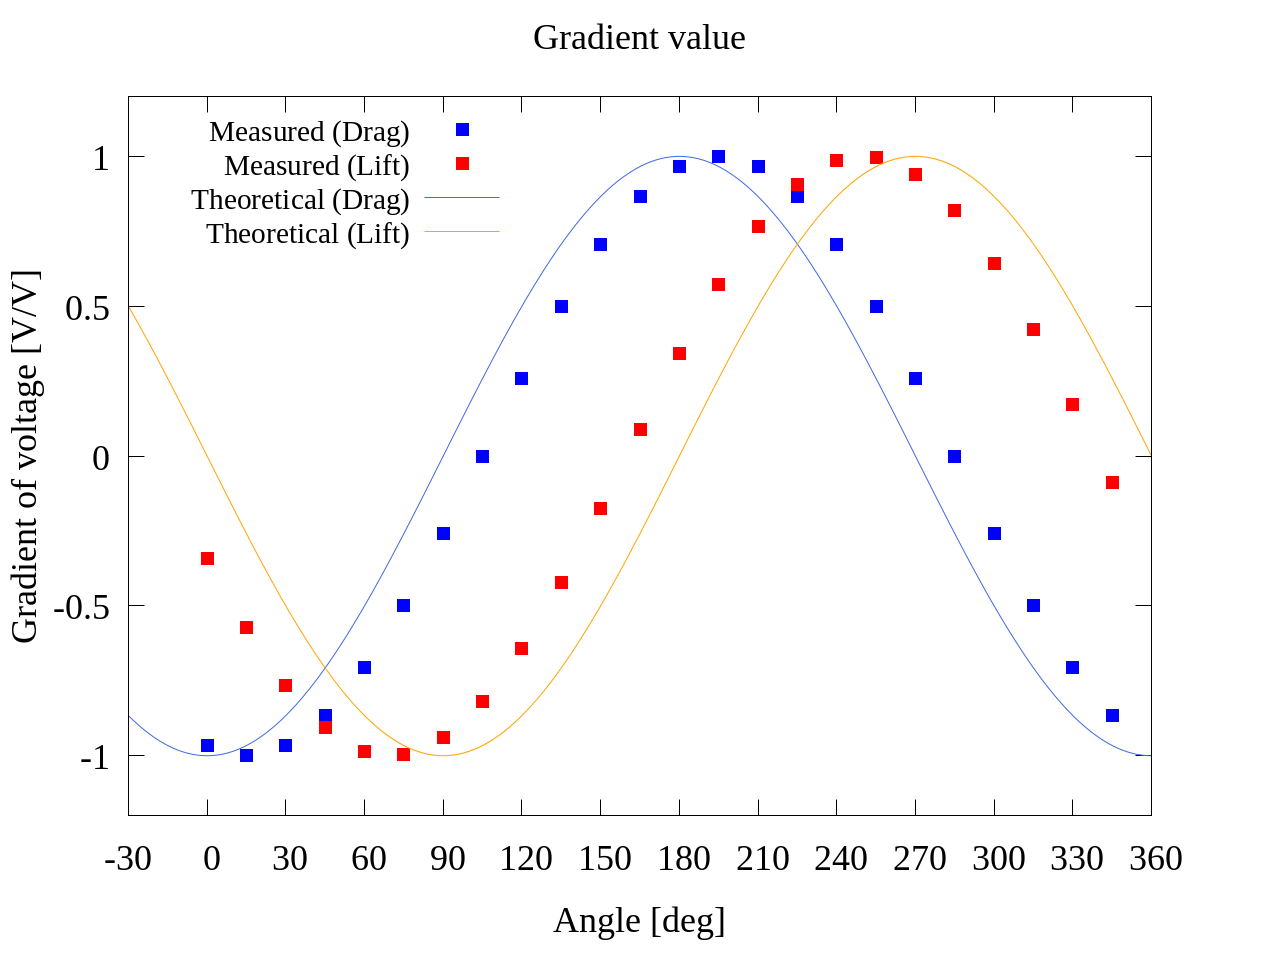
\includegraphics[width=65mm]{../../02_workspace/result/rotation_tx=15.0_tx=-20.0/plot/20/20_adjust-value.png}
            \caption{Simulated data [Case 2]}
            \includegraphics[width=65mm]{../../02_workspace/result/rotation_tx=15.0_tx=-20.0/plot/21/21-4_corrected_angle_drag.png}
            \caption{Corrected data (Drag) [Case 2]}
            \includegraphics[width=65mm]{../../02_workspace/result/rotation_tx=15.0_tx=-20.0/plot/21/21-4_corrected_angle_lift.png}
            \caption{Corrected data (Lift) [Case 2]}
        \end{center}
    \end{figure_here}

    \begin{figure_here}
        \subsubsection{テストデータ : Case 2}
        \vskip \baselineskip
        $\theta_{1 \mathrm{test}} = 90 \; \mathrm{[deg]}$, $\theta_{2 \mathrm{test}} = -90 \; \mathrm{[deg]}$
        \footnotesize
        \begin{center}
            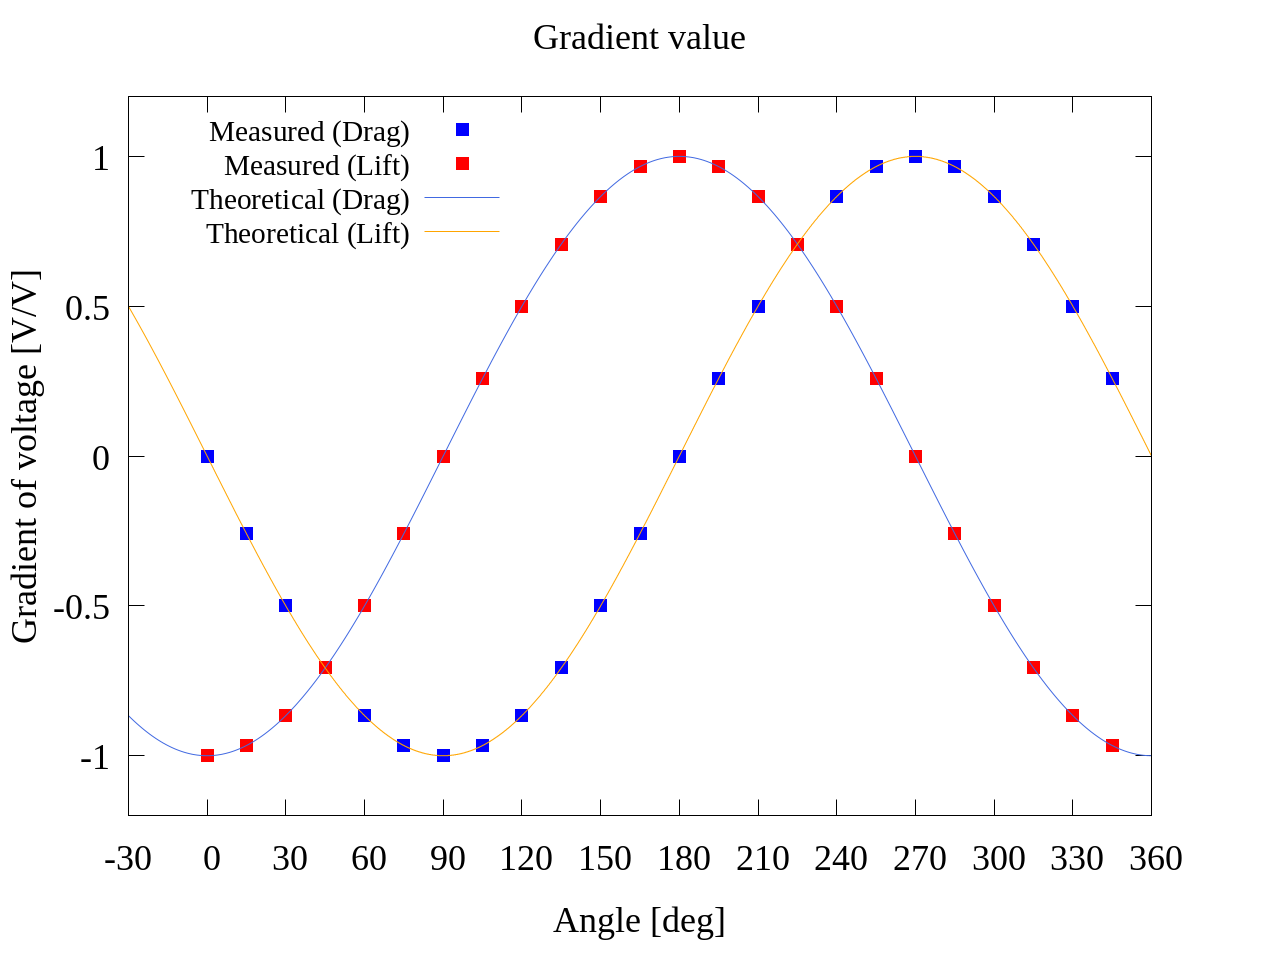
\includegraphics[width=65mm]{../../02_workspace/result/rotation_tx=90.0_tx=-90.0/plot/20/20_adjust-value.png}
            \caption{Simulated data [Case 2]}
            \includegraphics[width=65mm]{../../02_workspace/result/rotation_tx=90.0_tx=-90.0/plot/21/21-4_corrected_angle_drag.png}
            \caption{Corrected data (Drag) [Case 2]}
            \includegraphics[width=65mm]{../../02_workspace/result/rotation_tx=90.0_tx=-90.0/plot/21/21-4_corrected_angle_lift.png}
            \caption{Corrected data (Lift) [Case 2]}
        \end{center}
    \end{figure_here}
\end{multicols}

\subsection{座標系のオフセットにおける補正理論}

正規座標系と座標系[2]のオフセットの補正理論を説明する.


\subsection{複合状態における補正理論}

\subsection{推定理論}